%File: main.tex
% ReGate: Reason-Attributed Selective Grounding
% AAAI 2027 Submission
\documentclass[letterpaper]{article}
\usepackage[submission]{aaai2027}
\usepackage[hyphens]{url}
\usepackage{graphicx}
\graphicspath{{figures/}}
\urlstyle{rm}
\def\UrlFont{\rm}
\usepackage{natbib}
\frenchspacing
\usepackage{booktabs}
\usepackage{array}
\usepackage{amsmath}
\usepackage{amssymb}
\usepackage{xspace}

\pdfinfo{
/TemplateVersion (2027.1)
}

\setcounter{secnumdepth}{2}

\newcommand{\Bench}{\textsc{SelectGround-Bench}\xspace}
\newcommand{\Method}{\textsc{ReGate}\xspace}

%\title{ReGate: Metamorphic Counterfactual Supervision for Reason-Attributed Selective Grounding}
\title{ReGate: Mitigating Hallucinations in Visual Grounding via Metamorphic Counterfactual Supervision}
\author{Anonymous Submission}
\affiliations{}

\begin{document}
\maketitle

% \begin{abstract}
% Grounding models are usually evaluated when the requested referent is present, yet reliable systems must also recognize when a query conflicts with the image or when the target cannot be observed. We introduce \emph{reason-attributed selective grounding}, in which a model either returns a supported label and box or abstains with the evidence-specific cause---visual contradiction or target unavailability---assigned by deterministic construction. SelectGround-Bench converts existing annotations into $7{,}072$ training instances through seven deterministic relations, providing annotation-defined relation tests whose operators and reference outcomes are model-independent once the capability-controlled agricultural label space is fixed. Same-source groups place contrasting outcomes under shared provenance, making source identity alone insufficient for prediction. ReGate first adapts Qwen3-VL with the three-state grounding objective and then freezes the backbone to fit a compact routing gate. Native decoding after adaptation lowers false commitment from $0.211$ to $0.094$ on the comprehensive test and from $0.360$ to $0.155$ on source-disjoint PlantWild, while improving end-to-end mIoU from $0.656$ to $0.705$ in-domain and from $0.525$ to $0.645$ on image-disjoint RefCOCOg. The routed model reaches retention $0.976$, Strict-3 $0.856$, and FCA $0.132$; with a threshold selected exclusively on development data, it achieves $88.96\%$ test retention and $4.54\%$ FCA, reducing SFT-native FCA by $52.0\%$. On the comprehensive test, matched retraining raises metamorphic satisfaction from $0.527$ to $0.820$. Together, these results establish a selective-grounding paradigm in which deterministic evidence-state construction, representation adaptation, and explicit routing operate as complementary mechanisms.
% \end{abstract}
\begin{abstract}
Visual grounding models are typically trained under the assumption that the queried referent exists, causing unsupported localization when a query conflicts with the image or the target is unobservable. To address this problem, we propose ReGate: \emph{reason-attributed evidence gating}, a two-stage framework for selective grounding that either returns a supported label and box or abstains with an explicit cause: visual contradiction or target unavailability. At its core, ReGate employs \emph{metamorphic counterfactual supervision} (MCS), which turns seven deterministic relations into supervision by specifying how evidence states and spatial targets should remain invariant or change under controlled transformations. This construction yields SelectGround-Bench with $7{,}072$ training instances, construction-defined relation tests, and same-source counterfactual groups with contrasting outcomes under shared provenance. ReGate first adapts Qwen3-VL to the resulting three-state grounding objective and then fits a compact pre-decoding gate for explicit routing. Across six training-disjoint probes, ReGate delivers strong selective grounding and cross-domain transfer: a development-selected operating point reduces the SFT-native false-commitment rate by $52.0\%$ while increasing supported retention, and matched retraining raises metamorphic satisfaction from $0.527$ to $0.820$. On the comprehensive test, under the same instruction and output schema, ReGate also outperforms GPT-5.6 Sol in false commitment ($0.132$ versus $0.302$), Strict-3 accuracy, and end-to-end grounding. These results establish metamorphic counterfactual supervision as an effective and reusable supervision paradigm for evidence-aware VLM adaptation.
\end{abstract}



\section{Introduction}

Vision--language models (VLMs) can accurately localize natural-language expressions \citep{radford2021clip,li2023blip2,liu2023llava,wang2024qwen2vl,liu2023groundingdino}, but standard referring-expression benchmarks usually assume that the requested target exists and is visible \citep{mao2016refcocog}. When a query conflicts with the image, refers to an absent target, or lies outside the observable region, a model may still emit a plausible label and box: a spatially auditable but unsupported commitment that we term \emph{unsupported grounding hallucination}. Unlike mislocalizing a supported target, the correct action is to withhold localization.

To address this problem, we propose \Method: \emph{reason-attributed evidence gating}, for \emph{reason-attributed selective grounding}. \Method predicts \emph{supported grounding}, \emph{visual contradiction}, or \emph{target unavailable}; supported cases require a correct label and region, whereas unsupported cases require abstention with the corresponding cause. This three-state formulation extends binary answerability by determining both whether grounding is warranted and why it should be withheld, complementing strong localization models with an explicit evidence-state decision before localization.

A central challenge is to learn evidence distinctions rather than source identity. Independently collected negatives may expose scene, acquisition, or provenance shortcuts. This issue is especially demanding in agriculture, where fine-grained symptoms, small objects, role ambiguity, and target absence complicate the boundary between localization and abstention. We therefore introduce \emph{metamorphic counterfactual supervision} (MCS). Seven deterministic relations specify how wording, appearance, geometry, query compatibility, target visibility, and spatial annotations should remain invariant or change under controlled transformations \citep{chen1998metamorphic,segura2016survey}. Their instantiation, \Bench, produces annotation-defined supervision and relation tests; same-source counterfactual groups assign contrasting outcomes under shared provenance, directly supervising query--evidence compatibility. By reusing target-identity and localization annotations, %MCS also provides a scalable auxiliary task for VLM pretraining and adaptation.
MCS also offers a scalable auxiliary supervision task for VLM pretraining and adaptation.

\begin{figure*}[t]
\centering
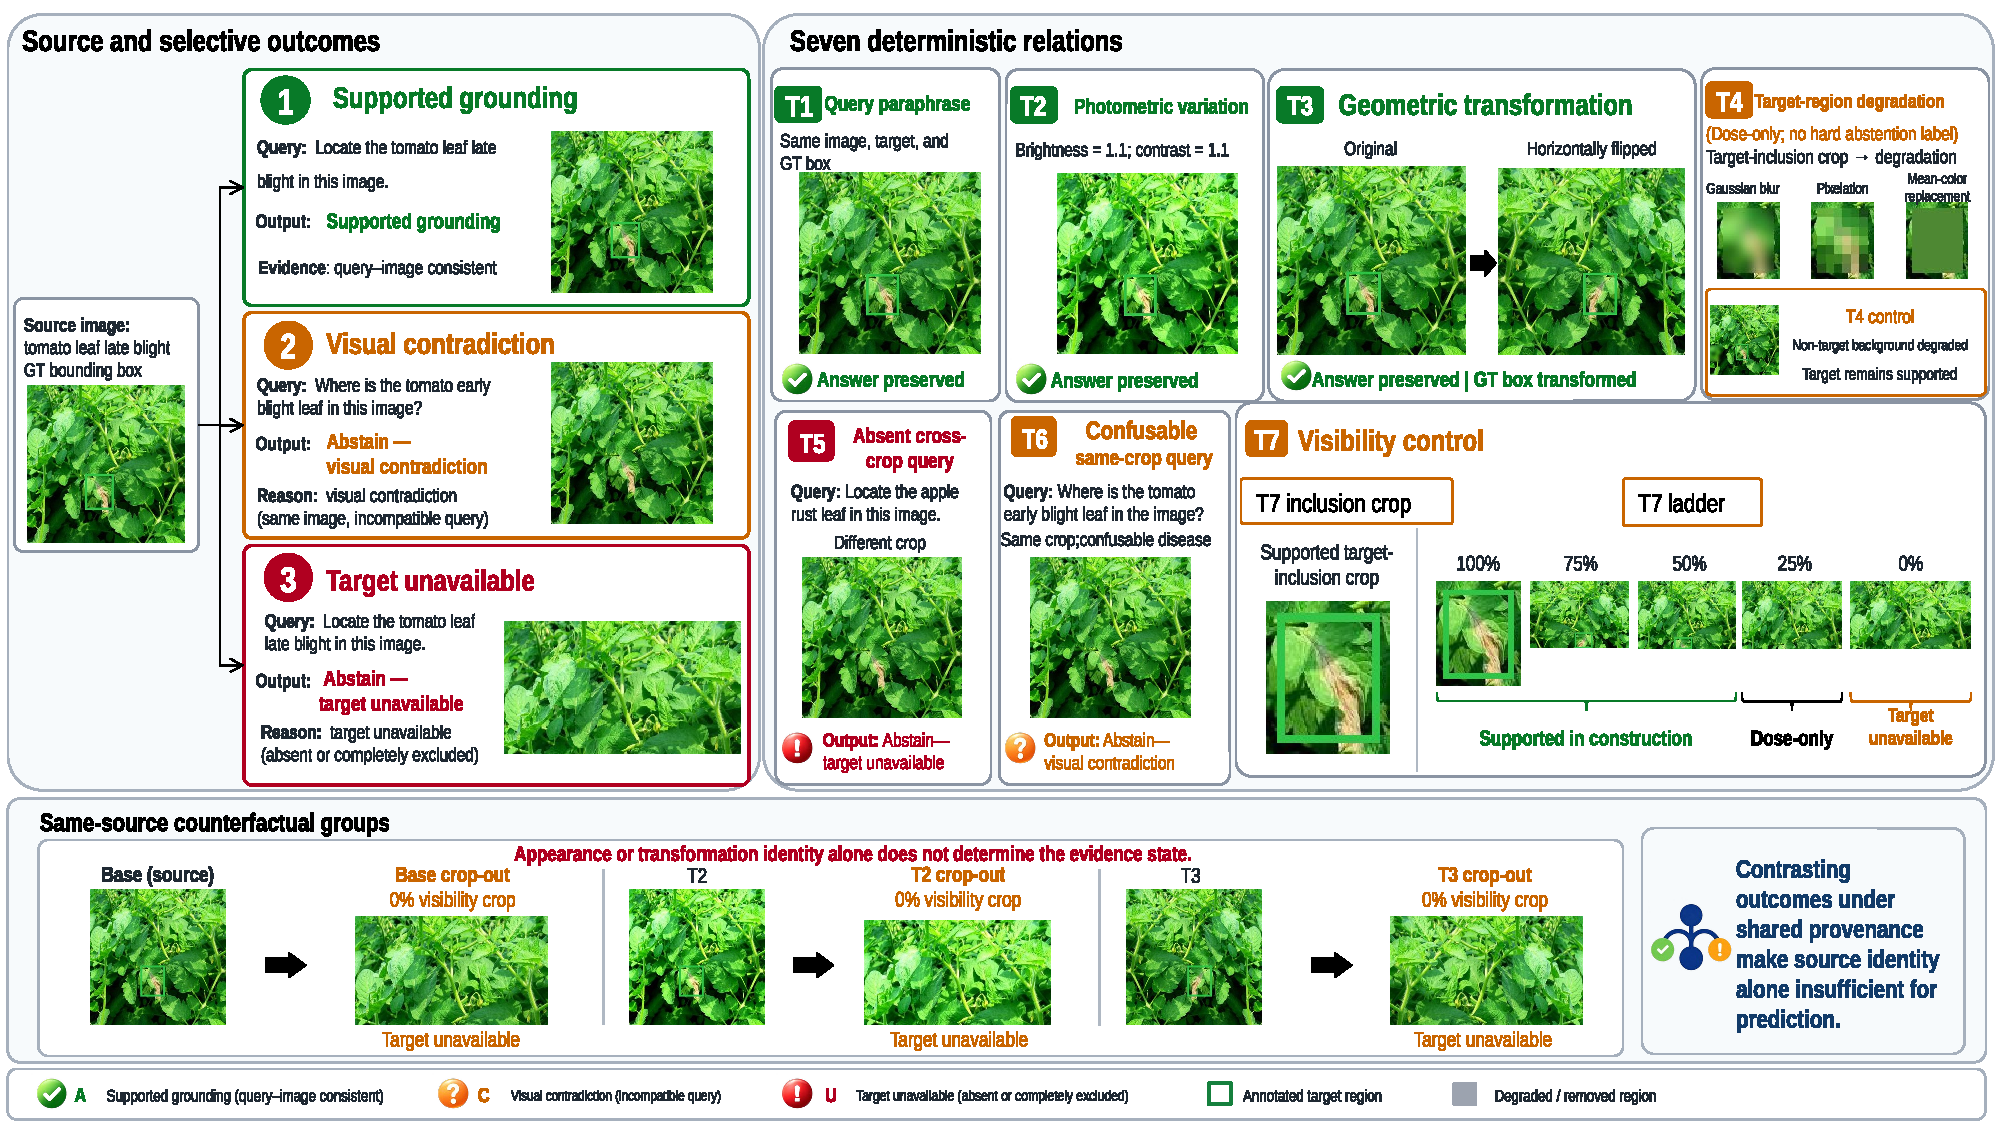
\includegraphics[width=0.95\textwidth]{figures/Fig1.pdf}
\caption{Task and benchmark construction. Same-source transformations yield supported grounding, visual contradiction, or target unavailability while controlling query compatibility and target visibility.}
\label{fig:motivation}
\end{figure*}

Built on Qwen3-VL-8B-Instruct, \Method first adapts the VLM for structured grounding and three-state prediction, then freezes the adapted backbone and fits a compact pre-decoding gate. The gate routes supported inputs to the shared grounding decoder and returns an explicit abstention reason otherwise, combining representation-level hallucination mitigation with high-retention routing.

Our contributions are threefold:
\begin{itemize}
\item We formulate unsupported grounding hallucination as an annotation-verifiable three-state problem unifying localization, contradiction detection, and target unavailability.
\item We introduce MCS and \Bench, deriving reusable evidence-state supervision and relation tests from seven deterministic transformations and same-source counterfactual groups.
\item We develop the two-stage \Method framework, which substantially reduces unsupported commitment while improving label-gated localization and supported retention.
\end{itemize}

Experiments span a comprehensive in-domain test, controlled probes, source-disjoint PlantWild, and image-disjoint RefCOCOg, comparing the frozen backbone, native post-adaptation decoding, and explicit routing; grouping, representation, evidence-removal, and visibility studies further isolate the gains. A development-selected operating point reduces SFT-native false commitment by $52.0\%$ while increasing retention, and matched retraining raises metamorphic satisfaction from $0.527$ to $0.820$. Under the same instruction and schema, \Method also outperforms GPT-5.6 Sol in false commitment ($0.132$ versus $0.302$), Strict-3, and end-to-end grounding.


\section{Related Work}

\textbf{Multimodal hallucination and unsupported visual queries.}
VLM hallucination includes objects, attributes, and relations that are unsupported by the visual input \citep{li2023pope,bai2024hallucinationsurvey}. POPE probes object hallucination through existence-oriented questions \citep{li2023pope}, while Antidote targets counterfactual-presupposition and object-perception hallucinations through synthetic post-training \citep{wu2025antidote}. Grounding has also been investigated as a hallucination remedy, yet stronger grounding does not automatically reduce hallucination in open-ended generation \citep{geigle2024grounding}. We focus on a spatially auditable failure: committing to a label and box when benchmark-defined evidence is contradictory or unavailable.

\textbf{Selective prediction and visual-evidence verification.}
Selective prediction controls the trade-off between coverage and predictive risk \citep{geifman2017selective,geifman2019selectivenet}. Reliable VQA extends this principle with learned selectors and answer-verification mechanisms \citep{whitehead2022reliable,dancette2023selective,khan2024consistency,srinivasan2024recoverr}. SIEVES explicitly scores localized visual evidence for selective prediction across out-of-distribution tasks \citep{rodriguez2026sieves}. These methods mainly estimate whether an answer should be trusted. \Method advances selective prediction into grounding by predicting one of three evidence states before localization and distinguishing annotation-defined visual contradiction from unavailable target evidence.

\textbf{Generalized and counterfactual grounding.}
Conventional referring-expression comprehension assumes that a valid target is present. GREC relaxes this assumption to allow zero, one, or multiple targets, and RECANTFormer addresses the resulting variable-target prediction problem \citep{he2023grec,hemanthage2024recantformer}. Counterfactual REC constructs queries whose referents cannot be found and learns a counterfactual label alongside localization \citep{yu2024counterfactualrec}. Together, these works establish that grounding should not force a region when the query lacks a valid referent. Our formulation extends this direction with first-class separation of visual contradiction and target unavailability, reason-attributed abstention, and strict evaluation under spatially transformed annotations.

\textbf{Counterfactual and metamorphic supervision.}
Counterfactual vision--language training uses minimally changed image--text pairs to improve fine-grained discrimination and compositional reasoning \citep{zhang2025cfvlm,wu2025antidote}. Metamorphic testing specifies expected output relations under controlled input transformations when a complete direct oracle is unavailable \citep{chen1998metamorphic,segura2016survey}. Relational validation across cyber--cyber digital twins further shows how controlled system variants can verify required properties under counterfactual behavior \citep{ahlgren2021facebook}. \Bench combines these principles through deterministic, annotation-defined transformations that intervene on query compatibility, target visibility, and evidence preservation while retaining source provenance. The resulting records support both sample-wise supervision and relation-stratified strict testing without generative counterfactual imagery.

\textbf{Agricultural visual diagnosis and grounding.}
Plant-disease recognition varies substantially in illumination, background, scale, and acquisition source \citep{mohanty2016plantvillage,plantdoc2019,wei2024plantwild}, while agricultural VLM and grounding resources increasingly evaluate multimodal reasoning and localization \citep{agrobench2025,agrigptvl2025,agrogpt2024,grefcw2026,agrovg2026}. These conditions make agriculture a natural stress test for all three evidence states and source shift, while COCO-derived training and RefCOCOg evaluation test transfer to general visual categories.

\section{\Bench}
\label{sec:benchmark}

\subsection{Task and Metamorphic Construction}
\label{sec:task}
\label{sec:transforms}

\Bench operationalizes metamorphic counterfactual learning by deriving evidence-state supervision from datasets with target-identity and location annotations. Given image $I$ and query $q$, the reference outcome is
$y^*\in\{\textsc{Answer}(l^*,b^*),\textsc{Abstain}(\rho^*)\}$, where $l^*$ is the target label, $b^*\in[0,1000]^4$, and $\rho^*$ is visual contradiction or target unavailability. A prediction $o$ yields a decision $d(o)$ and, when applicable, a label $l(o)$, box $b(o)$, or reason $\rho(o)$. Contradiction is assigned only when source annotations identify a configured confusable class while excluding the queried class. Construction-verified absence, an incompatible cross-crop query, or complete target removal yields unavailability. Thus, once the admissible label space is fixed, source annotations and deterministic transformations define every reference outcome independently of the evaluated model.

A fixed symmetric canonicalizer evaluates label equivalence, and invalid outputs receive no semantic, spatial, or reason credit. With $\mathsf{ans}=\textsc{Answer}$, $\mathsf{abs}=\textsc{Abstain}$, and $d=d(o)$, $l=l(o)$, $b=b(o)$, and $\rho=\rho(o)$, define
\begin{equation}
\begin{aligned}
C_S&=\mathbf 1[d=\mathsf{ans},l=l^*],%\qquad
C_R=\mathbf 1[d=\mathsf{abs},\rho=\rho^*],\\
C_G&=C_S\,\mathbf 1[\mathrm{IoU}(b,b^*)\geq0.5].
\end{aligned}
\label{eq:correctness}
\end{equation}

Figure~\ref{fig:motivation} summarizes the seven deterministic relations. T1--T3 preserve the target under paraphrasing, photometric variation, and geometric transformation. T4 varies target degradation, with a supported non-target degradation control. T5 pairs an observed crop with an absent cross-crop query; T6 substitutes a confusable same-crop class; and T7 controls retained target visibility. Base, photometric, and geometric appearances are additionally paired with complete crop-outs, preventing appearance or transformation identity from determining the state. Hard labels are used only when annotations and transformations determine the semantic and, when applicable, spatial outcome; other degradation and partial-visibility records are reserved for graded-response analysis.

T6 leaves the image unchanged and admits a substituted query only when it belongs to the fixed same-crop confusable set, is absent from all source-image annotations, and remains in the retained label space. T7 requests $100\%,75\%,50\%,25\%,$ and $0\%$ retained visibility and remaps the box into derived-image coordinates. The $100\%$, $75\%$, and nominal $50\%$ records achieving at least $50\%$ visibility are supported; complete exclusion is unavailable; the remaining intermediate records are graded only. A separate T7 inclusion crop retains the target with approximately $10\%$ surrounding context. %Complete operator and routing specifications appear in the Technical Supplement.

\subsection{Same-Source Data and Evaluation Protocol}
\label{sec:data_protocol}
\label{sec:pairing}
\label{sec:composition}
\label{sec:probes}

The principal contradiction and visibility records are grouped by source. T6 combines different queries with the same image, whereas T7 combines target-retaining and target-excluding views of the same annotation. Hence $\operatorname{src}(I_a)=\operatorname{src}(I_u)$ but $y_a\neq y_u$, making source identity insufficient within a group. The grouped subset contains $1{,}907$ instances: $372$ supported anchors, $973$ contradiction variants, and $281$ target-retaining plus $281$ target-excluding variants. Some anchors participate in both T6 and T7; the remaining records supply additional annotation-derived supervision.

Before resampling, the assembled training split contains $6{,}545$ instances and $6{,}138$ distinct records. Training-only resampling expands the $973$ contradiction instances to $1{,}500$, adding $527$ instances and yielding the $7{,}072$-instance composition in Table~\ref{tab:composition}; COCO-derived records use canonical categories, instances, and boxes \citep{lin2014coco}. The agricultural label space is fixed before splitting using the frozen base VLM on the verified PlantDoc pool: 20 of 24 observed categories meet the predefined category-level threshold of $0.40$ correct label-and-localization accuracy at IoU $0.5$. Categories are retained or excluded in full, without record-level filtering or downstream results, and the resulting universe is then split by source image. All derivatives of a source remain in one partition; dose-only records remain separate; and resampling follows group assignment.

\begin{table}[t]
\centering
\small
\setlength{\tabcolsep}{1mm}
\begin{tabular}{@{}>{\raggedright\arraybackslash}p{0.475\columnwidth}rcc@{}}
\toprule
Component & Count & Dec. & State \\
\midrule
Contradiction counterfactuals & 1,500 & Abs. & Contr. \\
Complete target exclusions & 669 & Abs. & Unavail. \\
Cross-crop unavailable queries & 1,500 & Abs. & Unavail. \\
Appearance-matched crop-outs & 200 & Abs. & Unavail. \\
COCO-derived unavailable & 500 & Abs. & Unavail. \\
COCO-derived supported & 1,100 & Ans. & Supp. \\
Visibility-controlled supported & 300 & Ans. & Supp. \\
Original/transformed supported & 1,303 & Ans. & Supp. \\
\midrule
Total & 7,072 & 38:62 & 2,703/1,500/2,869 \\
\bottomrule
\end{tabular}
\caption{Effective training composition after training-only resampling. In the total row, Dec.\ is Answer:Abstain and State is Supported/Contradiction/Unavailable.}
\label{tab:composition}
\end{table}

Table~\ref{tab:probes} summarizes six training-disjoint probes. The comprehensive probe evaluates all three states and eleven non-base relation variants. L1 isolates same-crop contradiction, and L2 pairs retained evidence with complete exclusion. L3 contains 750 visibility-controlled records: fixed-point metrics use 183 fully visible and 148 fully excluded endpoints, while the remaining 419 define the graded response. PlantWild \citep{wei2024plantwild} uses its official field-image test split and retains the 12 disease classes represented during SFT, producing 144 supported, 144 unavailable, and 120 contradictory records; its image-level annotations support selective-state and reason evaluation but not box scoring. RefCOCOg \citep{mao2016refcocog} contributes 181 original expressions, categories, and boxes, paired with 181 image-disjoint COCO images whose annotations exclude the queried category. COCO training images are disjoint from RefCOCOg evaluation images, and PlantWild is screened for exact and perceptual overlap.

\begin{table}[t]
\centering
\small
\setlength{\tabcolsep}{0.7mm}
\begin{tabular*}{\columnwidth}{@{\extracolsep{\fill}}lcl@{}}
\toprule
Probe & S/U & Evaluation focus \\
\midrule
L1    & 205/205     & Same-crop discrimination (T6) \\
L2    & 395/395     & Evidence retention/exclusion \\
L3    & 183/148     & $100\%/0\%$ endpoints; partial-level curve \\
Comp. & 1,323/1,323 & Comprehensive in-domain test \\
PW    & 144/264     & PlantWild source-disjoint field test \\
Ref.  & 181/181     & RefCOCOg image-disjoint grounding \\
\bottomrule
\end{tabular*}
\caption{Training-disjoint probes (S/U: supported/unsupported).}
\label{tab:probes}
\end{table}

\subsection{Metrics}
\label{sec:metrics}

Let $\mathcal D_{\mathrm{sup}}$ and $\mathcal D_{\mathrm{unsup}}$ denote the fixed supported and unsupported reference universes. The false-commitment rate (FCA) and supported retention $\mathrm{Ret}_S$ are the answer-selection rates on $\mathcal D_{\mathrm{unsup}}$ and $\mathcal D_{\mathrm{sup}}$, respectively; $\mathrm{A\_FU}=1-\mathrm{Ret}_S$. Selective MCC is the standard Matthews coefficient on the binary answer/non-answer decision. The two task-specific aggregate metrics are
\begin{align}
\mathrm{E2E\mbox{-}mIoU}
&=|\mathcal D_{\mathrm{sup}}|^{-1}
\sum_{i\in\mathcal D_{\mathrm{sup}}}
C_S(o_i)\,\mathrm{IoU}_0(b(o_i),b_i^*)\\
\mathrm{Strict\mbox{-}3}
&=\frac{\sum_{i\in\mathcal D_{\mathrm{sup}}}C_S(o_i)+
\sum_{i\in\mathcal D_{\mathrm{unsup}}}C_R(o_i)}
{|\mathcal D_{\mathrm{sup}}|+|\mathcal D_{\mathrm{unsup}}|}
\label{eq:metrics}
\end{align}
where $\mathrm{IoU}_0$ maps invalid boxes to zero. E2E-mIoU therefore jointly measures answering, label correctness, and localization, whereas Strict-3 measures three-state semantic correctness without localization.

For probe $p$, let $\mathcal V_p$ be its instantiated relation variants, $\mathcal D_{p,v}$ their records, and $m_v(o_i)$ strict compliance with the construction-defined semantic and spatial outcome. Macro metamorphic test satisfaction is
\begin{equation}
\operatorname{MTS}_p=
\frac{1}{|\mathcal V_p|}\sum_{v\in\mathcal V_p}
\frac{1}{|\mathcal D_{p,v}|}\sum_{i\in\mathcal D_{p,v}}m_v(o_i).
\label{eq:mts}
\end{equation}
MTS weights each variant equally and does not credit predictions that are mutually consistent but jointly incorrect. Supported relations require $C_G$; complete crop-outs require unavailability; T5 and T6 require their designated reasons; and supported T7 records additionally require the spatial criterion. L3 separately measures response across all available visibility levels.

For generative interfaces, a final invalid parse is a non-answer for selection metrics and receives no semantic, reason, or spatial credit. For \Method, the gate route defines binary selection: a malformed or abstention-form candidate on an answer route remains an answer selection but receives zero correctness credit. Supported answer-and-grounding accuracy and unsupported-reason accuracy are reported only as secondary decompositions in the construction contrast.

\section{Reason-Attributed Evidence Gating}
\label{sec:method}

MCS is model-independent at the level of construction operators and reference outcomes. \Method is a backbone-compatible two-stage framework for VLMs exposing a query-conditioned hidden representation and a structured grounding decoder; our implementation uses Qwen3-VL-8B-Instruct \citep{bai2025qwen3vl}. Stage~1 uses metamorphic evidence-state supervision to jointly adapt the VLM representation and an auxiliary state gate. Stage~2 freezes the adapted VLM, validates the readout position, and separately fits the inference gate on the resulting stationary representation. Supported inputs proceed to grounding generation, whereas unsupported inputs return the attributed cause without decoding. Figure~\ref{fig:framework} summarizes the framework.

\begin{figure*}[t]
\centering
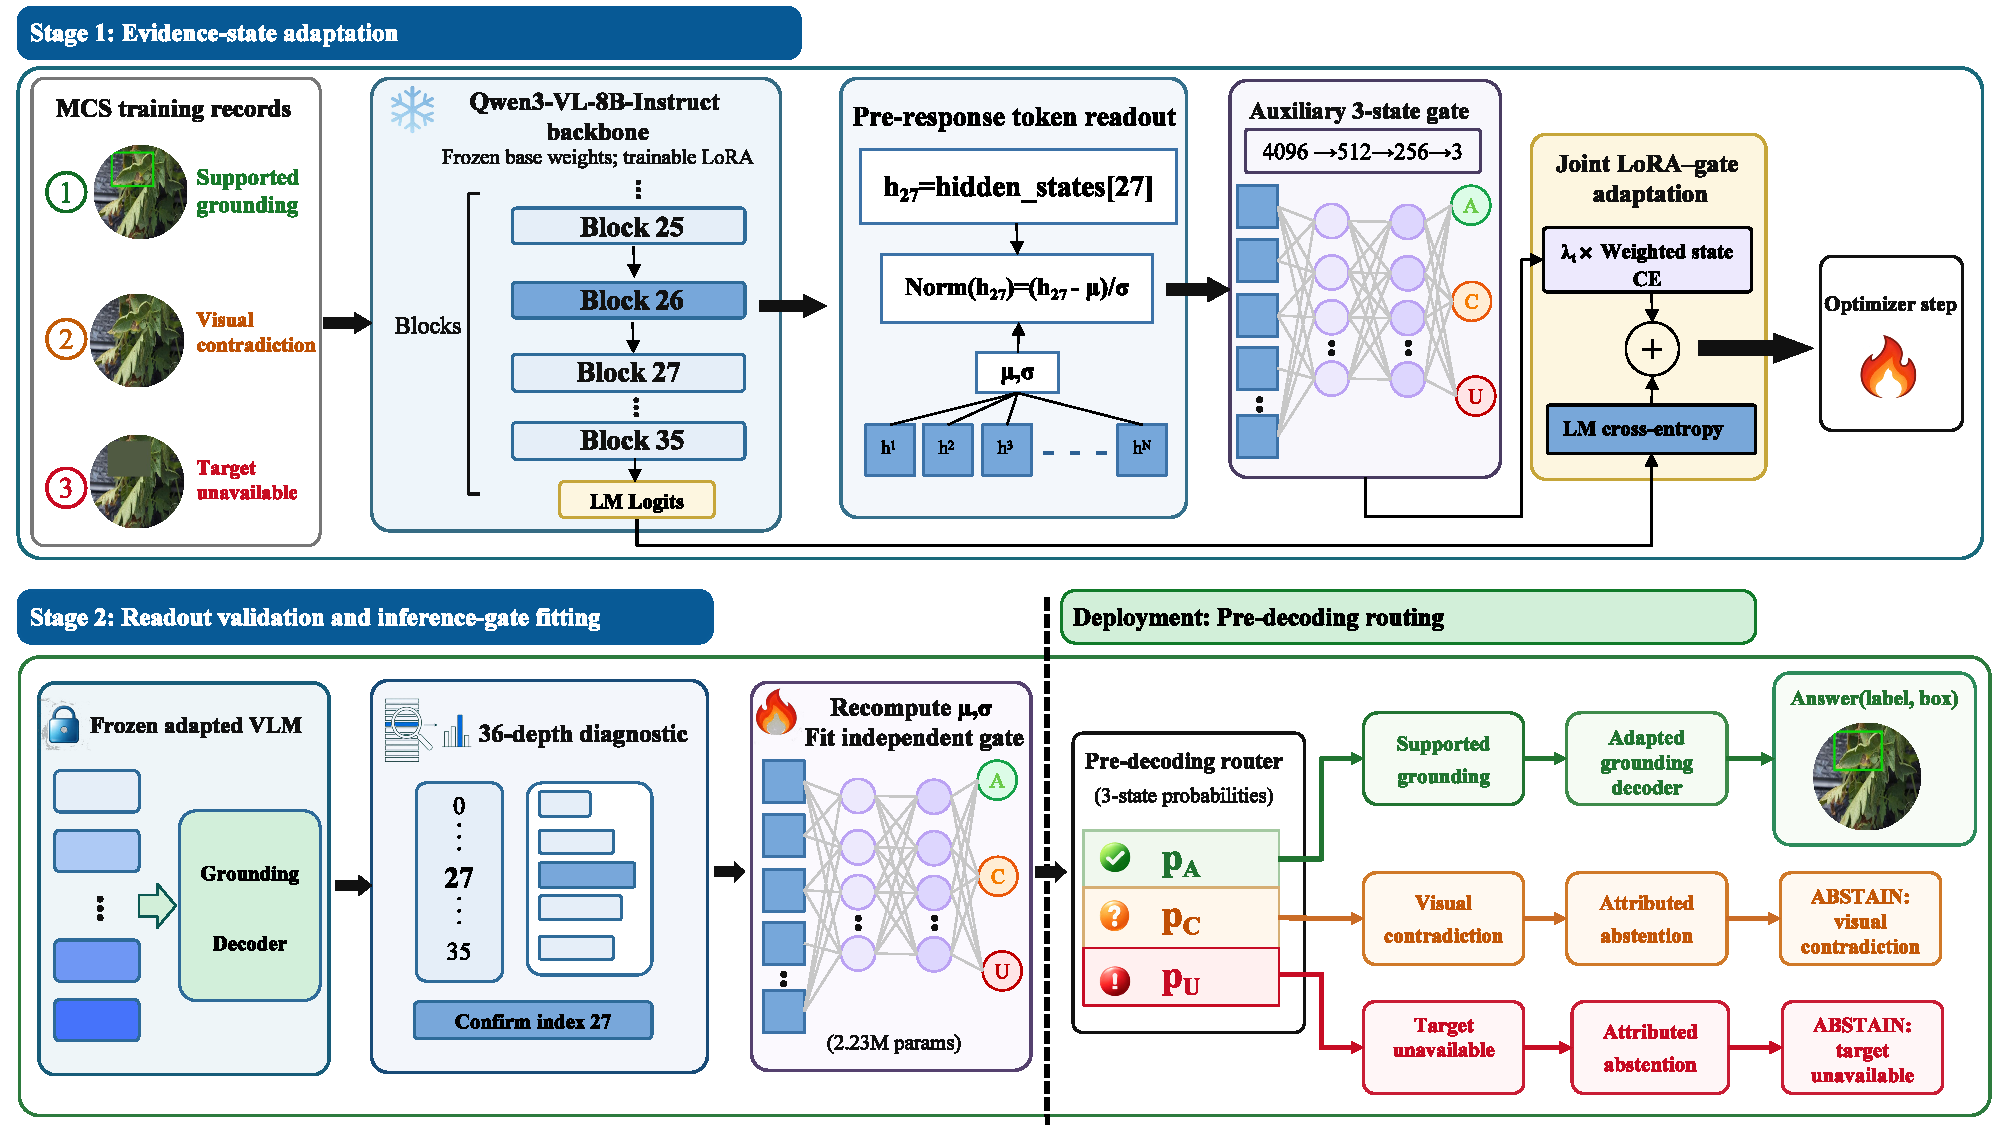
\includegraphics[width=0.95\textwidth]{figures/Fig2.pdf}
\caption{Two-stage \Method. Stage~1 jointly adapts LoRA and an auxiliary state gate; Stage~2 freezes the adapted VLM, confirms the layer-27 readout, and fits the parameterized inference gate for supported grounding or reason-attributed abstention.}
\label{fig:framework}
\end{figure*}

\subsection{Metamorphic Evidence-State Adaptation}
\label{sec:training}

For an image--query pair, the readout is the hidden state of the prompt token immediately preceding the first response token. Before joint adaptation, a matched-capacity depth study fits identical logistic probes at three evenly spaced API indices, 9, 18, and 27, using source-group-disjoint training-side diagnostic partitions; the development comparison selects index 27. Because index zero is the embedding output, this readout is the output of transformer block 26. Benchmark test records and external probes never enter this choice.

Let $\mathbf h_{27}$ denote the selected representation and $\mathbf z=\operatorname{Norm}(\mathbf h_{27})$, where Stage~1 normalization statistics are computed from frozen-backbone training representations. The auxiliary state gate is
%\begin{equation}
$\mathbf p_\phi=\operatorname{softmax}\!\left(g_\phi(\mathbf z)\right)$,
%\qquad
$\mathbf p_\phi=(p_{\phi,A},p_{\phi,C},p_{\phi,U})$,
%\label{eq:aux_gate}
%\end{equation}
where $A$, $C$, and $U$ denote Supported, Visual Contradiction, and Target Unavailable. The gate $g_\phi$ is a $4096\!\rightarrow\!512\!\rightarrow\!256\!\rightarrow\!3$ MLP with GELU activations and dropout $0.1$.

We adapt the backbone with LoRA \citep{hu2022lora} by% for up to six epochs using
\begin{equation}
%\begin{aligned}
\mathcal L_t=\mathcal L_{\mathrm{LM}}
-\lambda_tN^{-1}\sum_i w_{s_i}\log p_{\phi,s_i}%,\\
%\lambda_t&=0.4\min(1,t/10),\qquad
%\mathbf w=(1.0,1.5,1.0),
%\end{aligned}
\label{eq:loss}
\end{equation}
where $\lambda_t=0.4\min(1,t/10)$, $\mathbf w=(1.0,1.5,1.0)$, $t$ is the optimizer step, $\mathcal L_{\mathrm{LM}}$ is cross-entropy over the structured grounding or abstention response, $N$ is the minibatch size, and $\mathbf w$ orders the three states as $(A,C,U)$. Same-source counterfactual records encode the metamorphic structure directly in their evidence-state labels, enabling joint representation adaptation through standard sample-wise optimization without an additional pairwise objective. Among the six epoch checkpoints, we retain the checkpoint with minimum teacher-forced language-model loss on a fixed 100-record subset of the formal $2{,}408$-record development pool.

\subsection{Readout Validation and Inference-Gate Refit}
\label{sec:probing}

After adaptation, a separate source-group-disjoint diagnostic fits a logistic probe $P_\ell$ at each of the 36 transformer depths using $1{,}599$ probe-fitting and 137 probe-development records. Over states $\mathcal S=\{A,C,U\}$, it selects the layer with maximum worst-state validation accuracy:
\begin{equation}
m_\ell=\min_{c\in\mathcal S}\operatorname{Acc}_{\mathrm{val},c}(P_\ell),
\qquad
\ell^*=\arg\max_\ell m_\ell .
\label{eq:layer_selection}
\end{equation}
The scan independently confirms index 27 with $m_{27}=0.9574$. These probes use only training-side diagnostic records and do not enter gate fitting or inference.

We then freeze the selected backbone and grounding decoder, recompute normalization statistics from all adapted training representations, and fit an independently parameterized inference gate $g_\psi$ with the same MLP architecture using cross-entropy and development-set early stopping. The Stage~1 gate serves only as an auxiliary training head; Stage~2 does not reuse its parameters, and only $g_\psi$ supplies reported \Method decisions. This post-adaptation fit separates representation learning from final routing and estimates the deployed decision rule on the stationary adapted feature space.
This stage reuses the same evidence-state labels and introduces no additional supervision. Including biases, the inference gate has $2.23M$
%$2{,}229{,}763$ 
parameters, or $0.028\%$ of the backbone.

\subsection{Reason-Attributed Routing}
\label{sec:arch}

The final gate produces
$(p_A,p_C,p_U)=\operatorname{softmax}(g_\psi(\operatorname{Norm}(\mathbf h_{27})))$.
The default operating point predicts
$\hat s=\arg\max_{s\in\{A,C,U\}}p_s$, with ties involving $A$ resolved in favor of answering. A supported decision invokes the adapted grounding decoder with the shared structured instruction to generate a label and box; $C$ and $U$ directly return visual contradiction and target unavailability, respectively, without autoregressive grounding generation. For selective operation, thresholded routing answers when $p_A\geq\tau$ and otherwise chooses $\arg\max_{s\in\{C,U\}}p_s$. The reported low-FCA operating point selects $\tau$ exclusively on development data, while sweeping $\tau$ traces the FCA--retention curve.

\section{Experiments}
\label{sec:experiments}

We evaluate whether evidence-state adaptation reduces unsupported grounding, same-source construction produces compatibility-sensitive representations, and explicit routing transfers across datasets and decision interfaces.

\subsection{Experimental Setup}
\label{sec:exp_setup}

\textbf{Systems.}
\textbf{Base} is the frozen Qwen3-VL backbone with native structured decoding, \textbf{SFT native} applies the same decoder after Stage~1 adaptation, and \textbf{\Method} adds the Stage~2 gate. Base--SFT evaluates the complete adaptation pipeline: evidence-state data, joint language-model and state losses, and LoRA. SFT--\Method measures the effect of adding the deployed Stage~2 router while keeping the adapted backbone and grounding generator fixed. LoRA uses $r=16$, $\alpha=32$, dropout $0.05$, learning rate $10^{-4}$, and at most six epochs.

\textbf{Routing interfaces.}
Five generative interfaces use the same adapted backbone and generator. \textbf{Native LM} is SFT native with the base structured instruction; \textbf{Direct} enumerates the three decisions; \textbf{Reward} adds outcome-utility guidance; \textbf{R+E} further specifies evidence-preservation and evidence-change principles; and \textbf{S-CoT} requests staged support analysis before the same output schema. Across these interfaces, prompt examples, preprocessing, decoding, schema, parser, and evaluation denominators are fixed; only the routing instruction changes. \Method instead obtains the decision from its Stage~2 gate. GPT-5.6 Sol serves as a prompted general-purpose reference under the same task schema.
All numerical comparisons use the common three-state output space. GREC and RECANTFormer \citep{he2023grec,hemanthage2024recantformer} 
return an empty target set, while Counterfactual REC uses a single counterfactual label; their native outputs therefore do not distinguish visual contradiction from target unavailability.

\textbf{Evaluation protocol.}
We use the six probes in Table~\ref{tab:probes} and the metrics in Section~\ref{sec:metrics}. The Grouped/Independent comparison retrains the complete pipeline with matched backbone, objective, state counts, and optimization. 
Additional details, including prompt strings, computing environment, source-separation procedures, full FCA--retention curves, and uncertainty estimates are provided in the supplement.
%Additional implementation details, including FCA--retention curves, and uncertainty analyses are provided in the supplement.

\subsection{Main Results}
\label{sec:fixed_point_comparison}

\begin{table}[t]
\centering
\small
\setlength{\tabcolsep}{1mm}
\begin{tabular*}{\columnwidth}{@{\extracolsep{\fill}}llrrrr@{}}
\toprule
Dataset & Interface & FCA$\downarrow$ & Ret.$\uparrow$ & S3$\uparrow$ & E2E$\uparrow$ \\
\midrule
Comprehensive & Base & 0.211 & 0.833 & 0.660 & 0.656 \\
 & SFT native & \textbf{0.094} & 0.851 & 0.819 & \textbf{0.705} \\
 & \Method & 0.132 & \textbf{0.976} & \textbf{0.856} & 0.701 \\
\midrule
PlantWild & Base & 0.360 & 0.792 & 0.375 & -- \\
 & SFT native & \textbf{0.155} & 0.764 & 0.647 & -- \\
 & \Method & 0.269 & \textbf{0.854} & \textbf{0.694} & -- \\
\midrule
RefCOCOg & Base & \textbf{0.044} & 0.983 & 0.762 & 0.525 \\
 & SFT native & \textbf{0.044} & 0.901 & \textbf{0.834} & \textbf{0.645} \\
 & \Method & 0.083 & \textbf{1.000} & 0.820 & \textbf{0.645} \\
\bottomrule
\end{tabular*}
\caption{Base--SFT--\Method comparison at fixed operating points. Ret., S3, and E2E denote supported retention, Strict-3, and E2E-mIoU; PlantWild has no box annotations.}
\label{tab:main_results}
\end{table}

\textbf{Evidence-state adaptation.}
Stage~1 lowers FCA from $0.211$ to $0.094$ on the comprehensive test and from $0.360$ to $0.155$ on PlantWild, while preserving $0.044$ on RefCOCOg. It simultaneously improves E2E-mIoU from $0.656$ to $0.705$ in-domain and from $0.525$ to $0.645$ on image-disjoint RefCOCOg (Table~\ref{tab:main_results}), enhancing label-gated localization while transferring hallucination mitigation to natural field imagery.

\textbf{High-retention routing.}
With the adapted backbone and generator fixed, the argmax gate raises comprehensive-test retention from $0.851$ to $0.976$, MCC from $0.758$ to $0.849$, and Strict-3 from $0.819$ to $0.856$, while reducing A\_FU from $0.149$ to $0.024$. 
%Its corresponding FCA is $0.132$, compared with $0.094$ for SFT native, revealing the complementary operating profiles of native adaptation and explicit routing.
This argmax operating point prioritizes supported coverage, reaching $0.976$ retention with FCA $0.132$; the development-selected threshold below provides the lower-FCA operating point.

\textbf{Development-selected operation.}
Selecting $\tau=0.9888$ exclusively on all $2{,}408$ development records at matched $86.05\%$ development retention yields $88.96\%$ test retention and $4.54\%$ FCA, compared with $85.11\%$ retention and $9.45\%$ FCA for SFT native. Development-selected routing therefore increases supported coverage while reducing false commitment by $52.0\%$. All fixed \Method entries use three-class argmax; this thresholded point is reported separately.

\subsection{Construction and Evidence Analyses}
\label{sec:diagnostic_probes}
\label{sec:grouping_ablation}

\textbf{Same-source construction.}
We compare Grouped training with independently sampled, category-constrained negatives through matched full retraining. The two conditions preserve supported records, state counts, targets, category--state strata, objective, architecture, and hyperparameters, and each fits its own final gate.

\begin{table}[t]
\centering
\small
\setlength{\tabcolsep}{0.7mm}
\begin{tabular*}{\columnwidth}{@{\extracolsep{\fill}}lrrrr@{}}
\toprule
Probe/interface & MTS$\uparrow$ & MCC$\uparrow$ & FCA$\downarrow$ & A\_FU$\downarrow$ \\
\midrule
Comp.-Gate & .820/.527 & .849/.523 & .132/.486 & .024/.045 \\
Comp.-Native & .807/.756 & .758/.660 & .094/.193 & .149/.148 \\
Ref.-Gate & .812/.867 & .920/.940 & .083/.055 & .000/.006 \\
Ref.-Native & .826/.876 & .858/.923 & .044/.039 & .099/.039 \\
PW-Gate & .673/.619 & .560/.350 & .269/.250 & .146/.396 \\
PW-Native & .648/.608 & .602/.449 & .155/.322 & .236/.208 \\
L1-Gate & .651/.502 & .393/.085 & .615/.766 & .059/.166 \\
L2-Gate & .622/.410 & .570/.091 & .476/.878 & .018/.068 \\
L3-Gate & .804/.502 & .836/.318 & .176/.831 & .011/.000 \\
\bottomrule
\end{tabular*}
\caption{Matched construction contrast. Cells report Grouped/Independent. Comp., Ref., and PW denote Comprehensive, RefCOCOg, and PlantWild.}
\label{tab:grouping_ablation}
\end{table}

Under the matched seed-42 protocol, Grouped training raises comprehensive-test Strict-3 from $0.663$ to $0.856$, retention from $0.955$ to $0.976$, supported answer-and-grounding accuracy from $0.762$ to $0.794$, unsupported-reason accuracy from $0.504$ to $0.865$, and the T6 pass rate from $0.263$ to $0.571$. It also reduces PlantWild A\_FU from $0.396$ to $0.146$ and raises retention from $0.604$ to $0.854$. Independent negatives remain competitive on RefCOCOg, whereas Grouped training produces the largest gains on the compatibility-controlled and source-disjoint probes (Table~\ref{tab:grouping_ablation}), validating same-source construction for reason-attributed decisions.

\textbf{Representation readout.}
Using identical source-group-disjoint train/development/test partitions and the same classifier over five probe-fitting seeds with the base backbone frozen, the pre-response prompt token reaches MCC $0.769\pm0.020$, compared with $0.363\pm0.011$ for visual-token mean, $0.337\pm0.009$ for visual-token max, and $0.115\pm0.029$ for visual query-attention. It is the strongest tested readout; the separate post-adaptation depth scan selects index 27.

\textbf{Controlled evidence response.}
The probes isolate fine-grained same-crop contradiction (L1 FCA $0.615$), complete evidence removal (L2 FCA $0.476$), and graded visibility (L3 MCC/FCA $0.836/0.176$). Among the balanced $395/395$ L2 records, source-instance and target-label matching after deduplication yields 148 complete target-retaining/target-removal pairs. Removing the target lowers $p_A$ by $0.786$ on average (95\% CI $[0.720,0.840]$), with the expected direction in $96.6\%$ of pairs. Across 183 L3 groups, $p_A$ increases with retained visibility (Spearman $\rho=0.750$, Kendall $\tau=0.682$); $78.6\%$ of adjacent levels are correctly ordered, corresponding to a $21.4\%$ violation rate (Fig.~\ref{fig:visibility_response}). The L2 fixed-point FCA complements this probability-level analysis by testing whether the response crosses the final decision boundary.

\begin{figure}[t]
\centering
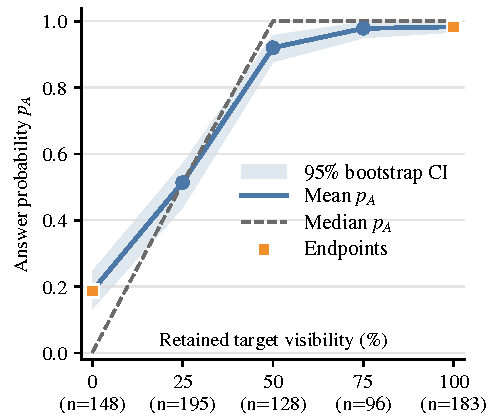
\includegraphics[
  width=0.95\columnwidth,
  height=0.64\columnwidth
]{figures/checkpoint444_visibility_response.pdf}
\caption{L3 visibility response. Mean and median $p_A$ increase with retained target visibility; shading shows the 95\% source-instance-group bootstrap CI, and orange markers denote the hard-evaluation endpoints.}
\label{fig:visibility_response}
\end{figure}

\textbf{Relation-level consistency.}
The strict-pass vector is T1 paraphrase $0.818$; T2 photometric/crop-out $0.798/0.938$; T3 geometry/crop-out $0.808/0.913$; T4 control $0.831$; T5 absent query $0.948$; T6 confusable query $0.571$; T7 inclusion/ladder $0.750/0.781$; and base crop-out $0.859$, yielding macro MTS $0.820$. Joint success on the supported T4 control and unavailable crop-outs confirms state-specific behavior across transformations. The most demanding relation,  T6, demonstrates discrimination among fine-grained same-crop alternatives.% and is the most demanding relation.

\subsection{Routing Interfaces and Generalization}
\label{sec:plantwild}
\label{sec:gpt56_comparison}

\textbf{Routing-interface comparison.}

\begin{table}[t]
\centering
\small
\setlength{\tabcolsep}{1.5mm}
\begin{tabular*}{\columnwidth}{@{\extracolsep{\fill}}lccc@{}}
\toprule
Interface & Comprehensive & RefCOCOg & PlantWild \\
\midrule
\Method & \textbf{.849/.024/.856} & \textbf{.920/.000}/.820 & .560/\textbf{.146}/.694 \\
Native LM & .758/.149/.819 & .858/.099/\textbf{.834} & \textbf{.602}/.236/.647 \\
Direct & .724/.198/.844 & .862/.127/.693 & .581/.250/\textbf{.755} \\
Reward & .703/.162/.834 & .838/.127/.588 & .506/.208/.645 \\
R+E & .696/.180/.832 & .768/.204/.627 & .513/.222/.679 \\
S-CoT & .637/.357/.765 & .685/.343/.572 & .545/.417/.642 \\
\bottomrule
\end{tabular*}
\caption{Routing interfaces results on %. Each cell reports 
MCC/A\_FU/Strict-3.%; bold marks the best result for each dataset and metric.
}
\label{tab:routing_interfaces}
\end{table}

\Method leads six of nine dataset--metric comparisons: all three comprehensive metrics, RefCOCOg MCC and A\_FU, and PlantWild A\_FU (Table~\ref{tab:routing_interfaces}). Native LM leads RefCOCOg Strict-3 and PlantWild MCC, while Direct leads PlantWild Strict-3. Overall, explicit evidence gating provides the strongest cross-dataset routing profile.

\textbf{Source-disjoint transfer.}
On source-disjoint PlantWild, \Method reaches state-specific strict accuracies of $0.750/0.317/0.951$ for supported grounding, visual contradiction, and target unavailability. The strong supported and unavailable results confirm transfer to natural field imagery, while the contradiction score establishes fine-grained same-crop discrimination as the benchmark's most demanding transfer test.

\textbf{General-purpose reference.}
Table~\ref{tab:gpt56_full} compares the complete two-stage \Method system with prompted GPT-5.6 Sol on all six probes. The comparison uses identical records, task schema, parser, and ground-truth denominators; GPT-5.6 Sol receives the Native-LM instruction and per-record query of \Method's supported route. The same fixed instruction is retained on RefCOCOg without dataset-specific prompt tuning.

\begin{table}[t]
\centering
\small
\setlength{\tabcolsep}{1mm}
\begin{tabular*}{\columnwidth}{@{\extracolsep{\fill}}lccccc@{}}
\toprule
Probe & FCA$\downarrow$ & A\_FU$\downarrow$ & MCC$\uparrow$ & S3$\uparrow$ & E2E$\uparrow$ \\
\midrule
Comp. & .132/.302 & .024/.076 & .849/.639 & .856/.664 & .701/.625 \\
L1 & .615/.576 & .059/.102 & .393/.365 & .651/.649 & .810/.614 \\
L2 & .476/.570 & .018/.073 & .570/.411 & .682/.656 & .641/.573 \\
L3 & .176/.338 & .011/.077 & .836/.615 & .807/.785 & .689/.657 \\
Ref. & .083/.088 & .000/.000 & .920/.915 & .820/.677 & .645/.446 \\
PW & .269/.223 & .146/.167 & .560/.587 & .694/.463 & --/-- \\
\bottomrule
\end{tabular*}
\caption{\Method/GPT-5.6 Sol comparison; cells follow this order. S3 and E2E denote Strict-3 and E2E-mIoU.}
\label{tab:gpt56_full}
\end{table}

On the comprehensive test, \Method/GPT-5.6 Sol/SFT native attain A\_FU $0.024/0.076/0.149$ and MCC $0.849/0.639/0.758$; \Method and SFT native also exceed the prompted reference in E2E-mIoU. Paired 95\% intervals favor \Method over GPT-5.6 Sol for comprehensive-test FCA, A\_FU, Strict-3, and E2E-mIoU. The L1 and PlantWild FCA intervals overlap, while paired intervals favor \Method for L1 E2E-mIoU, L2/L3 FCA, and RefCOCOg Strict-3 and E2E-mIoU. These results establish strong transfer under a shared-prompt protocol and a consistent advantage on the comprehensive evaluation.

\section{Conclusion}

%We introduce reason-attributed selective grounding and an annotation-defined construction framework based on deterministic relations, including explicit same-source counterfactual groups. Stage~1 substantially reduces unsupported commitment and improves label-gated localization, while the 2.23M-parameter Stage~2 gate delivers high-retention routing with explicit reasons and, on the comprehensive test, a development-selected operating point that raises retention while halving FCA relative to SFT native. Across matched retraining, controlled evidence interventions, relation-level tests, source-disjoint evaluations, and the shared-prompt GPT-5.6 comparison, \Method consistently delivers compatibility-sensitive, evidence-responsive decisions. By turning existing localization annotations into reusable evidence-state supervision, the construction also offers a scalable auxiliary pretraining task for future VLMs. \Method establishes a practical foundation for grounding systems that localize when supported and abstain with an attributable reason otherwise, together with a readily transferable design for future adaptation to additional backbones and visual categories.

% We introduced reason-attributed selective grounding, metamorphic counterfactual supervision, and the two-stage \Method framework. MCS turns deterministic same-source relations into annotation-defined supervision for supported grounding, visual contradiction, and target unavailability. \Method couples representation adaptation with compact pre-decoding routing: Stage~1 reduces unsupported commitment and improves label-gated localization, while Stage~2 provides high-retention routing and a development-selected operating point that halves FCA relative to SFT native while increasing retention. Matched construction studies, controlled evidence interventions, source-disjoint transfer, and the shared-prompt GPT-5.6 comparison demonstrate compatibility-sensitive, evidence-responsive decisions. By deriving reusable supervision from existing localization annotations, MCS offers a scalable auxiliary task for VLM pretraining, while \Method provides a backbone-compatible foundation for extending selective grounding to additional models and visual domains.

We introduced reason-attributed selective grounding, metamorphic counterfactual supervision (MCS), and the two-stage \Method framework. MCS converts deterministic same-source relations into annotation-defined supervision for supported grounding, visual contradiction, and target unavailability. \Method combines representation adaptation with compact pre-decoding routing: Stage~1 reduces unsupported commitment and improves label-gated localization, while Stage~2 enables high-retention routing and a development-selected operating point that halves FCA versus SFT native while increasing retention. Matched construction studies, controlled evidence interventions, source-disjoint transfer, and a shared-prompt GPT-5.6 comparison demonstrate compatibility-sensitive, evidence-responsive decisions. By reusing existing localization annotations, MCS provides a scalable auxiliary task for VLM pretraining, while \Method offers a backbone-compatible foundation for extending selective grounding across models and visual domains.

{\small\bibliography{aaai2027}}

\end{document}
